\cleardoublepage
\setcounter{chapter}{3} %The counter for chapters should be set one less than 
                        %the actual chapter number, for example, {1} for 
                        %chapter 2, and {2} for chapter 3.
\setcounter{section}{4} %The counter for sections should be set to match the
                        %actual chapter number, for example, {2} for sections 
                        %in chapter, and {3} for sections in chapter 3. 
\chapter{GUI Features}
\markboth{WEBGUI USERS' GUIDE}{GUI FEATURES}
\pagenumbering{arabic}
\setcounter{page}{39} %The counter for page numbers must be placed here in your
                     %chapter, following the \chapter and \markboth commands.
                     %It should always be the next available right-hand page.
                     %All chapters start on new rights. It will always be
                     %an odd number.  

 
\section{Basic layout}
\begin{figure}[H]
\centering
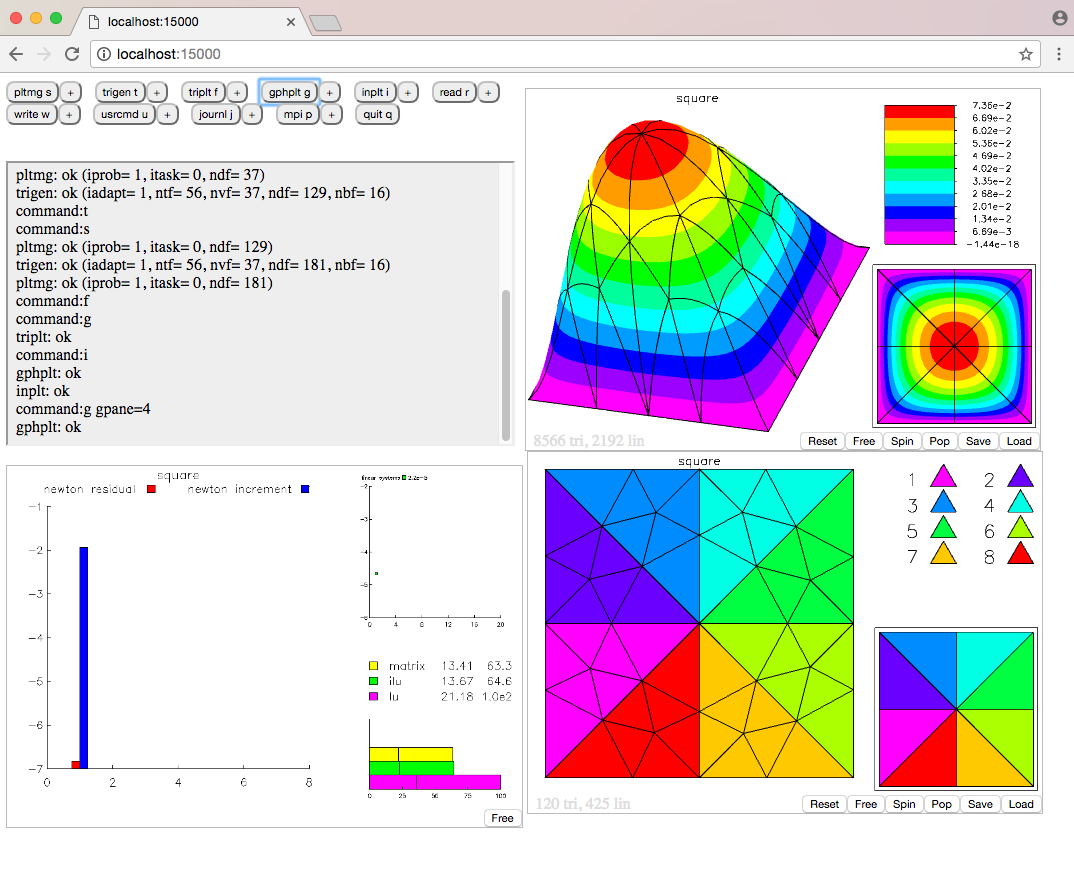
\includegraphics[width=0.75\textwidth]{pix/example2.png}
\caption{\f{WEBGUI}'s appearance in a web browser.}
\label{fig:4-1}
\end{figure} 
Above is an image of \f{WEBGUI} running together with Randolph Bank's software \f{PLTMG}. This picture illustrates
the basic features of \f{WEBGUI}'s graphic user interface. Randy's softare \f{PLTMG} called \textbf{webinit}
to define 11 buttons and many parameters and options. (To learn how to add buttons see Section \ref{sec:3-2}.)
Next it called \textbf{webstart}. After that a user opened a web browser and directed it to the host computer's URL. 
Then the user clicked some buttons issuing commands. \f{PLTMG} outputted many lines of text and one 2D
image and two 3D objects.

The web browser graphic interface is divided into 4 rectangle areas. The top left area contains the command buttons
and a pane to display text output. The text output pane also displays a history of the commands issued. A command is
issued whenever the user (i) presses a command button, (ii) closes a drop down menu after 
changing a parameter, or (iii) types a command into the command string field and hits enter. (If you wish for
your software to send text output to the text output pane, use the routine \textbf{webwriteline} described in Section 
\ref{sec:2-2}.)

The remaining 3 rectangle areas are panes numbered 0, 1, 2 (corresponding to the top right, bottom left, and 
bottom right pane)(they are also numbered 3, 4, 5). These panes are where 2D images and 3D objects (WebGL) 
outputted by software are displayed. Each
pane can display either one 2D image or one 3D object. Whenever a new image or object is sent to a pane, the old
image or object disappears and is replaced. (If you wish your software to send 2D images to a display pane, see Section 
\ref{sec:2-3}. To send 3D objects to a display pane, see Section \ref{sec:2-4}.)

\section{Display panes}
\label{sec:4-4}
The web browser interface has 3 display panes. Each display one 2D image or one 3D object. The display panes 
are numbered 0, 1, 2 corresponding to the top right, bottom left, bottom right (also numbered 3, 4, 5). In Figure \ref{fig:4-1},
pane 0(3) and 2(5) contain a 3D object. And pane 1(4) contains a 2D image.

3D objects are displayed using WebGL 1.0. Most web browsers and computers from the year 2010 onward have WebGL enabled
by default. When a 3D object is displayed, the user can rotate, pan, and zoom the object using their mouse. Rotate
using the left mouse button, pan using the middle mouse button, and zoom using the right mouse button. If your mouse
doesn't have a center button, you can push the "option" (on Mac) or "alt" (on Windows) key while using the left mouse button 
instead. If your mouse doesn't have a right button, you can push the "command" (on Mac) or "windows" (on Windows) key 
while using the left mouse button instead.

\begin{center}
\begin{tabular}{|l|l|l|l|}
\hline
\multicolumn{2}{|c|}{\strutul Display pane buttons} \\
\hline 
\strutul
Button & Effect \\
\hline
\strutu
RESET & return a zoomed / panned / rotated image to its initial state \\
FREE & clear the image and free associated memory \\
SPIN & spin image \\
POP & place canvas in its own web browser tab\\
PUSH & return canvas to its original location in the web browser tab\\
SAVE & save image to a file\\
LOAD & read image from a file\\
\hline
\end{tabular}
\end{center}

Under each 3D object are 6 buttons labeled Reset, Free, Spin, Pop, Save, and Load. Pressing the Reset button
returns the 3D object to its original location reseting any rotation, pan, or zoom information. 

Pressing Free, deletes the object and frees any memory associated with storing the object. See Section 
\ref{sec:5-1} to learn about \f{WEBGUI}'s memory usage. 

Pressing Spin allows the object to rotate freely. It will continue rotating in the direction that the user
last rotated. After pressing Spin, you will see a new button labeled Stop. Pressing Stop stops the object from rotating
freely. 

Pressing Pop places the current display pane in its own browser tab or window (depending on your web 
browser's settings). If your web browser places the pane in a new tab but you prefer a new window, either 
change your web browser's settings or open a new window and cut and paste the tab's URL into the new window.
When a display pane resides in its own tab or window, you will see a button labeled Push under the new pane. 
Pressing Push will put the display pane back into the main controls window.

Pressing Save will save a binary file with an extension of "gpu" to your local computer containing the 3D object's information.
This file can be loaded back into a display pane using the Load button.

Under each 2D image is only 1 button labeled Free. Pressing this button deletes the image and frees any memory
associated with storing the image. See Section \ref{sec:5-1} to learn about \f{WEBGUI}'s memory usage. 

\section{Quaternion rotation}
3D objects that are drawn to frame 5 can be rotated, panned, and zoomed with the mouse (explained in previous section). 
Objects in frames 1, 2, 3, 4 cannot.
Frame 5's viewing area is a cube with the coordinates of the lower left back $(0,0,0)$ and the upper right front $(1,1,1)$.
The center of this frame is coordinates $(0.5,0.5,0.5)$. See Figure \ref{fig:4-3}.

\begin{figure}[H]
\centering
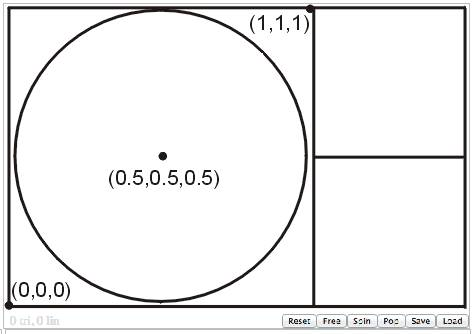
\includegraphics[width=0.75\textwidth]{pix/circle.jpg}
\caption{A 2D projection of a sphere in frame 5}
\label{fig:4-3}
\end{figure}

\begin{figure}[H]
\centering
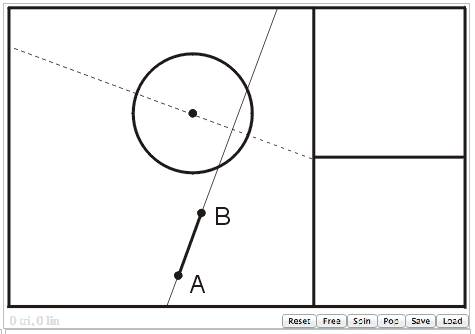
\includegraphics[width=0.75\textwidth]{pix/axis3.jpg}
\caption{Moving the mouse from $A$ to $B$ rotates the object in 3D around the dotted line axis.}
\label{fig:4-4}
\end{figure}

A 3D object gets rotated whenever a user depresses the left mouse button, moves the mouse, and then releases the
left mouse button. Rotation is calculated as follows. Imagine a sphere of radius $0.5$ that fills frame 5 with
center at $(0.5,0.5,0.5)$. Projected into 2D, this is a circle as shown in Figure \ref{fig:4-3}. The user can zoom and 
pan frame 5 moving the circle to a new size and location in the web browser. When a user depresses the left mouse button, 
call this point $A$. Then the user moves the mouse. Call the point where the user releases the left mouse button point $B$.
Projected into 2D, the line through the center of the circle perpendicular to line $AB$ is the axis
of 3D rotation. The axis is the dotted line in Figure \ref{fig:4-4}.

In 3D, the angle between the axis of rotation
and the $XY$ plane is $\alpha = sin^{-1}(d/r)$ where $r$ is the radius of the circle and 
$d$ is the distance between the center of the circle and
the line $AB$. If $d>r$ then $\alpha = \pi/2$. The above defines the axis of rotation $u$.
The amount of rotation in radians is $\theta = 3s/(2r)$ where $s$ is the distance from $A$ to $B$ and $r$ is the radius
of the circle. The associated quaternion to facilatate this rotation is 
$q=[cos(\theta /2), u_x sin(\theta /2), u_y sin(\theta /2), u_z sin(\theta /2)]$ when $u$ is normalized to length 1.

As the user holds down the left mouse button and moves the mouse between point $A$ and point $B$,
the mouse travels through points $C_k$ in between. For each point $C_k$, \f{WEBGUI} shows the user what the object would
look like if the user released the left mouse button at $C_k$. Therefore as the mouse moves, the object
appears to continually rotate. None-the-less, when the mouse button is released, the inbetween points $C_k$ are ignored
and the above formula is used to calculate the new orientation of the object.



\section{Control keys}
\label{sec:4-1}
\f{WEBGUI} has some features which are toggled with key strokes.
\begin{center}
\begin{tabular}{|l|l|l|l|}
\hline
\multicolumn{2}{|c|}{\strutul Control keys} \\
\hline 
\strutul
Key & Feature \\
\hline
\strutu
OPTION + C & toggles between command buttons and command text field \\
OPTION + I & toggles displaying rotation, pan, and zoom information \\
OPTION + R & toggles whether 3D objects inherit rotation, pan, and zoom\\
OPTION + W & toggles between 2 display panes wide and 1 pane wide \\
OPTION + F & toggles firewall on and off\\
OPTION + E & toggles endian flip on and off\\
OPTION + SAVE & saves 3D object as text instead of binary\\
\hline
\end{tabular}
\end{center}

To use the above features, you hold down the OPTION key while pressing the indicated key. On a Windows machine,
hold down the ALT key instead of the OPTION key.

OPTION + C toggles between command buttons and command text field. If your software calls \textbf{webinit} before
calling \textbf{webstart}, then your web browser GUI will have command buttons. Note that the command buttons are just
short cuts for generating and submitting command strings to the command string buffer. See Section \ref{sec:3-3} for an 
explanation. Therefore the buttons are never needed. If you prefer to type your own command strings, then you can
toggle the command buttons off and on with OPTION +C.

OPTION + I toggles displaying rotation, pan, and zoom information. When these keys are pressed, the 3D object display
pane that is in focus will display its current rotation, pan, and zoom information. Note that when a display pane contains
a 2D image, there is no rotation, pan, and zoom information to display for that display pane.

OPTION + R toggles whether 3D objects inherit the rotation, pan, and zoom setting from the previously displayed 3D object.
By default, when you display a new 3D object, it will display without any zoom, pan, or rotation applied even if you zoomed, 
panned, and rotated the previous 3D object that was in the same display pane. After you press OPTION + R, the web
browser will display a pop up message indicating the status of inheritance.

OPTION + W toggles the web browser's appearance between 2 display panes wide and 1 display pane wide. On mobile
devices the default is 1 display pane wide. On other devices the default is 2 display panes wide.

OPTION + F toggles the firewall on and off. When the firewall is activated, the bottom of the web browser will display the 
following line of text indicating this
\begin{verbatim}
FIREWALL ON: Only your ip address (X.X.X.X) can access webgui.
\end{verbatim}
and, on the server machine, the standard output will display
\begin{verbatim}
webgui: Only accepting ip address = X.X.X.X
\end{verbatim}
where x.x.x.x is your ip address. And when the firewall is turned off, the standard output will display
\begin{verbatim}
webgui: Accepting all ip addresses.
\end{verbatim}

OPTION + E toggles an endian flip on and off. All but one feature of \f{WEBGUI} are independent of whether the
server machine and client machine have the same endianness or not. The only feature that is affected is displaying
3D objects. 3D objects are sent between the server and client as a binary stream of 4 byte variables (either integers
or floating point numbers). By default, the client assumes that the server has the same endianness as itself. If this 
is not the case, then press OPTION + E, to toggle an endian flip to allow the correct display of 3D objects. When endian
flip is turned on, the bottom of the web browser will display the following line of text indicating this
\begin{verbatim}
ENDIAN FLIP: Client is receiving flipped endianness of server.
\end{verbatim}

OPTION + SAVE allows your computer to save a 3D object as ASCII text instead of a binary string of floating point
numbers. This allows you to view the 3D object and see the individual triangles and lines that make up the 
object. You can also view the colors of these triangles and lines. Currently, the Load button will not load the ASCII text
files. If you want to be able to load a saved 3D object, then press SAVE without holding down OPTION. This will
save the 3D object as a binary file and allow it to be loaded later.

\section{Miscelleanous}
\subsection{Display without controls}
\label{sec:4-2}

\f{WEBGUI} can be used another way. Instead of receiving user input and displaying software output, \f{WEBGUI}
can just be used to display output as show in Figure \ref{fig:4-2}. Notice how this is different than the normal appearance
in Figure \ref{fig:4-1}. To have your web browser perform this way, use the URL = "http:// localhost:15000/ sg?x=0" instead of 
URL = "http:// localhost:15000/ index.html". In place of $x=0$, choose $x=0$, $x=1$, or $x=2$ depending on which display pane 
you wish to view. And of course in place of "http:// localhost", you put the ip address of the host machine and in place of 
15000, you put the port that your web server is listening on. 

\begin{figure}[H]
\centering
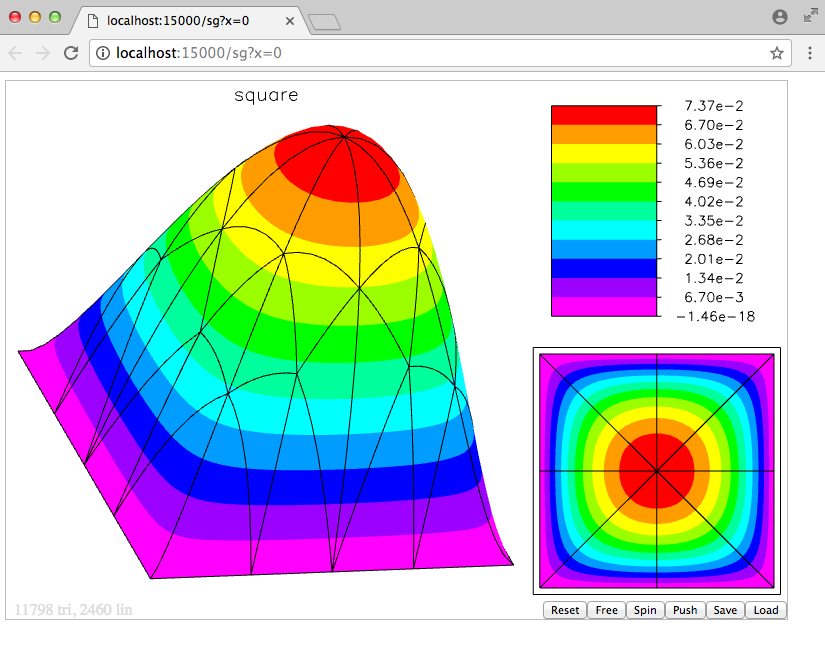
\includegraphics[width=0.75\textwidth]{pix/sg.png}
\caption{\f{WEBGUI} in display only mode by using a special URL.}
\label{fig:4-2}
\end{figure} 

\subsection{Save and view webpage offline}
\label{sec:4-3}

When you are viewing \f{WEBGUI} within your web browser, you may desire to save the web page so that you can 
view or edit the webpage offline. Of course at any time you can just select "Save page as" in your web browser. You can
even select "Save webpage complete". However if you do either of these and then open the saved files, they will not display
any 3D objects. If you wish to save a version that contains the 3D objects, there is a work around.

In your web browser, change the URL from "http:// localhost:15000/ index.html" to "http:// localhost:15000/ save". Of course
in place of "http:// localhost", you put the ip address of the host machine and in place of 15000, you put the port
that your web server is listening on. After entering this new URL, you will see what looks like the same web page. However,
if you choose "Save webpage complete" and reload it offline, you will see the 3D objects. This works because the 3D objects
will be stored as ASCII text data within a JavaScript file. This is recognized by your web browser and your web browser will
save it. Normally, the 3D objects are being stored as proprietary binary data which is must faster to transmit and load. But your
web browser does not recognize these binary files and won't save them. Only use the special save URL to save the web page;
\f{WEBGUI} will not operate correctly in save mode.

If you wish to save the appearance of a single 3D object (without the command buttons showing as displayed in Figure \ref{fig:4-2}), 
you have two choices. You can simply click the Save button
beneath the object you wish to save as explained in Section \ref{sec:4-4}. This saves a very small binary file. Or instead, 
you can go to the URL = "http:// localhost:15000/ save?x=0" which will allow you to view display pane 0 and save it by selecting
"Save webpage complete" from your web browser. Use $x=1$ or $x=2$ for display panes 1 and 2.

